\section{Comparative Evaluation}
\label{sec:eval}
\subsection{Setup and Metrics}
\label{sec:setup}
The November 16 evaluation covers 21 categories and five description levels. The main comparison, Group B, uses 265 shared prompts, with 53 per level and one delivered output per system per prompt. All BrickForma outputs in Group B are raw generations from its Q8\_0 weights. Group A contains 260 matched prompts for BrickGPT and BrickNet. Together the two groups contain 1,315 LDraw exports (Figure~\ref{fig:comparison-cohorts}).

\emph{Text--image alignment.}
Each export is rendered with uniform yellow material in eight $512{\times}512$ orthographic views, at azimuths spaced $45^\circ$ apart and at $25^\circ$ elevation. Each alignment score takes the maximum over views and is then averaged over prompts. VQAScore~\cite{vqascore} uses the first-token probability of \textquotedblleft Yes\textquotedblright\ from Qwen2.5-VL-7B-Instruct~\cite{qwen25vl}. PE~\cite{pe} uses cosine similarity of normalized image and text embeddings, and SigLIP2~\cite{siglip2} uses the sigmoid of the image--text logit.

\emph{Invalid placements.}
For an export with $n$ placements in file order, let $I_i$ indicate whether placement $i$ is invalid given the preceding placements under BrickNet's inset collision kernel~\cite{bricknet}. We compute $P_{\mathrm{inv}}=n^{-1}\sum_{i=1}^{n}I_i$ per export and report its mean across prompts.

\subsection{Main Results}
\begin{table}[t]
\centering\small
\setlength{\tabcolsep}{3pt}
\begin{tabular}{lrrrr}
\toprule
System & $P_{\mathrm{inv}}\downarrow$ & VQAScore $\uparrow$ & PE $\uparrow$ & SigLIP2 $\uparrow$ \\
\midrule
BrickForma & 0.81\% & \textbf{0.1079} & \textbf{0.1572} & \textbf{0.0565} \\
BrickGPT & \textbf{0.00\%} & 0.0926 & 0.1459 & 0.0262 \\
BrickNet & 17.88\% & 0.0259 & 0.1173 & 0.0016 \\
\bottomrule
\end{tabular}
\caption{Group B means on 265 matched prompts. BrickForma uses delivered raw outputs. Bold marks the best mean.}
\label{tab:main}
\end{table}

BrickForma attains the highest mean VQAScore (0.1079), PE (0.1572), and SigLIP2 (0.0565) on Group B (Table~\ref{tab:main}). It exceeds BrickGPT on 188, 166, and 168 of the 265 prompts for these metrics, respectively. The six paired alignment comparisons pass Holm correction under both tests (Appendix~\ref{app:eval}). BrickGPT has the lowest mean $P_{\mathrm{inv}}$ (0.00\%), followed by BrickForma (0.81\%) and BrickNet (17.88\%). Figures~\ref{fig:comparison-means} and~\ref{fig:comparison-distributions} show the means and score distributions.

\subsection{Performance across Description Levels}
\begin{table*}[t]
\centering\small
\setlength{\tabcolsep}{3pt}
\begin{tabular}{lrrlrrrr}
\toprule
Level & $n$ & Words & System & $P_{\mathrm{inv}}\downarrow$ & VQAScore $\uparrow$ & PE $\uparrow$ & SigLIP2 $\uparrow$ \\
\midrule
L1 & 53 & 13.4 & BrickForma & 0.41\% & 0.1841 & \textbf{0.1409} & \textbf{0.0254} \\
 &  &  & BrickGPT & \textbf{0.00\%} & \textbf{0.1911} & 0.1323 & 0.0132 \\
 &  &  & BrickNet & 15.14\% & 0.0445 & 0.1032 & 0.0002 \\
\midrule
L2 & 53 & 26.4 & BrickForma & 0.78\% & \textbf{0.1651} & \textbf{0.1453} & \textbf{0.0241} \\
 &  &  & BrickGPT & \textbf{0.00\%} & 0.1354 & 0.1391 & 0.0206 \\
 &  &  & BrickNet & 17.74\% & 0.0579 & 0.1037 & 0.0013 \\
\midrule
L3 & 53 & 37.3 & BrickForma & 0.73\% & \textbf{0.1467} & \textbf{0.1479} & \textbf{0.0717} \\
 &  &  & BrickGPT & \textbf{0.00\%} & 0.1061 & 0.1396 & 0.0199 \\
 &  &  & BrickNet & 23.30\% & 0.0211 & 0.1075 & 0.0012 \\
\midrule
L4 & 53 & 52.3 & BrickForma & 1.38\% & \textbf{0.0239} & \textbf{0.1792} & \textbf{0.0914} \\
 &  &  & BrickGPT & \textbf{0.00\%} & 0.0198 & 0.1609 & 0.0487 \\
 &  &  & BrickNet & 18.68\% & 0.0023 & 0.1344 & 0.0016 \\
\midrule
L5 & 53 & 78.6 & BrickForma & 0.75\% & \textbf{0.0198} & \textbf{0.1727} & \textbf{0.0698} \\
 &  &  & BrickGPT & \textbf{0.00\%} & 0.0107 & 0.1575 & 0.0286 \\
 &  &  & BrickNet & 14.56\% & 0.0035 & 0.1379 & 0.0035 \\
\bottomrule
\end{tabular}
\caption{Group B means by description level. Each level contains 53 prompts per system. Words is the mean English word count. Bold marks the best mean.}
\label{tab:levels}
\end{table*}

BrickForma leads PE and SigLIP2 at all five levels and VQAScore at L2--L5 (Table~\ref{tab:levels} and Figure~\ref{fig:comparison-levels}). At L1, the prompts average 13.4 words. BrickGPT scores 0.1911 on VQAScore and BrickForma scores 0.1841. BrickGPT has the lowest mean $P_{\mathrm{inv}}$ at each level. Figure~\ref{fig:gallery} shows two L1 and two L2 examples under matched rendering conditions.
\begin{figure*}[t]
\centering
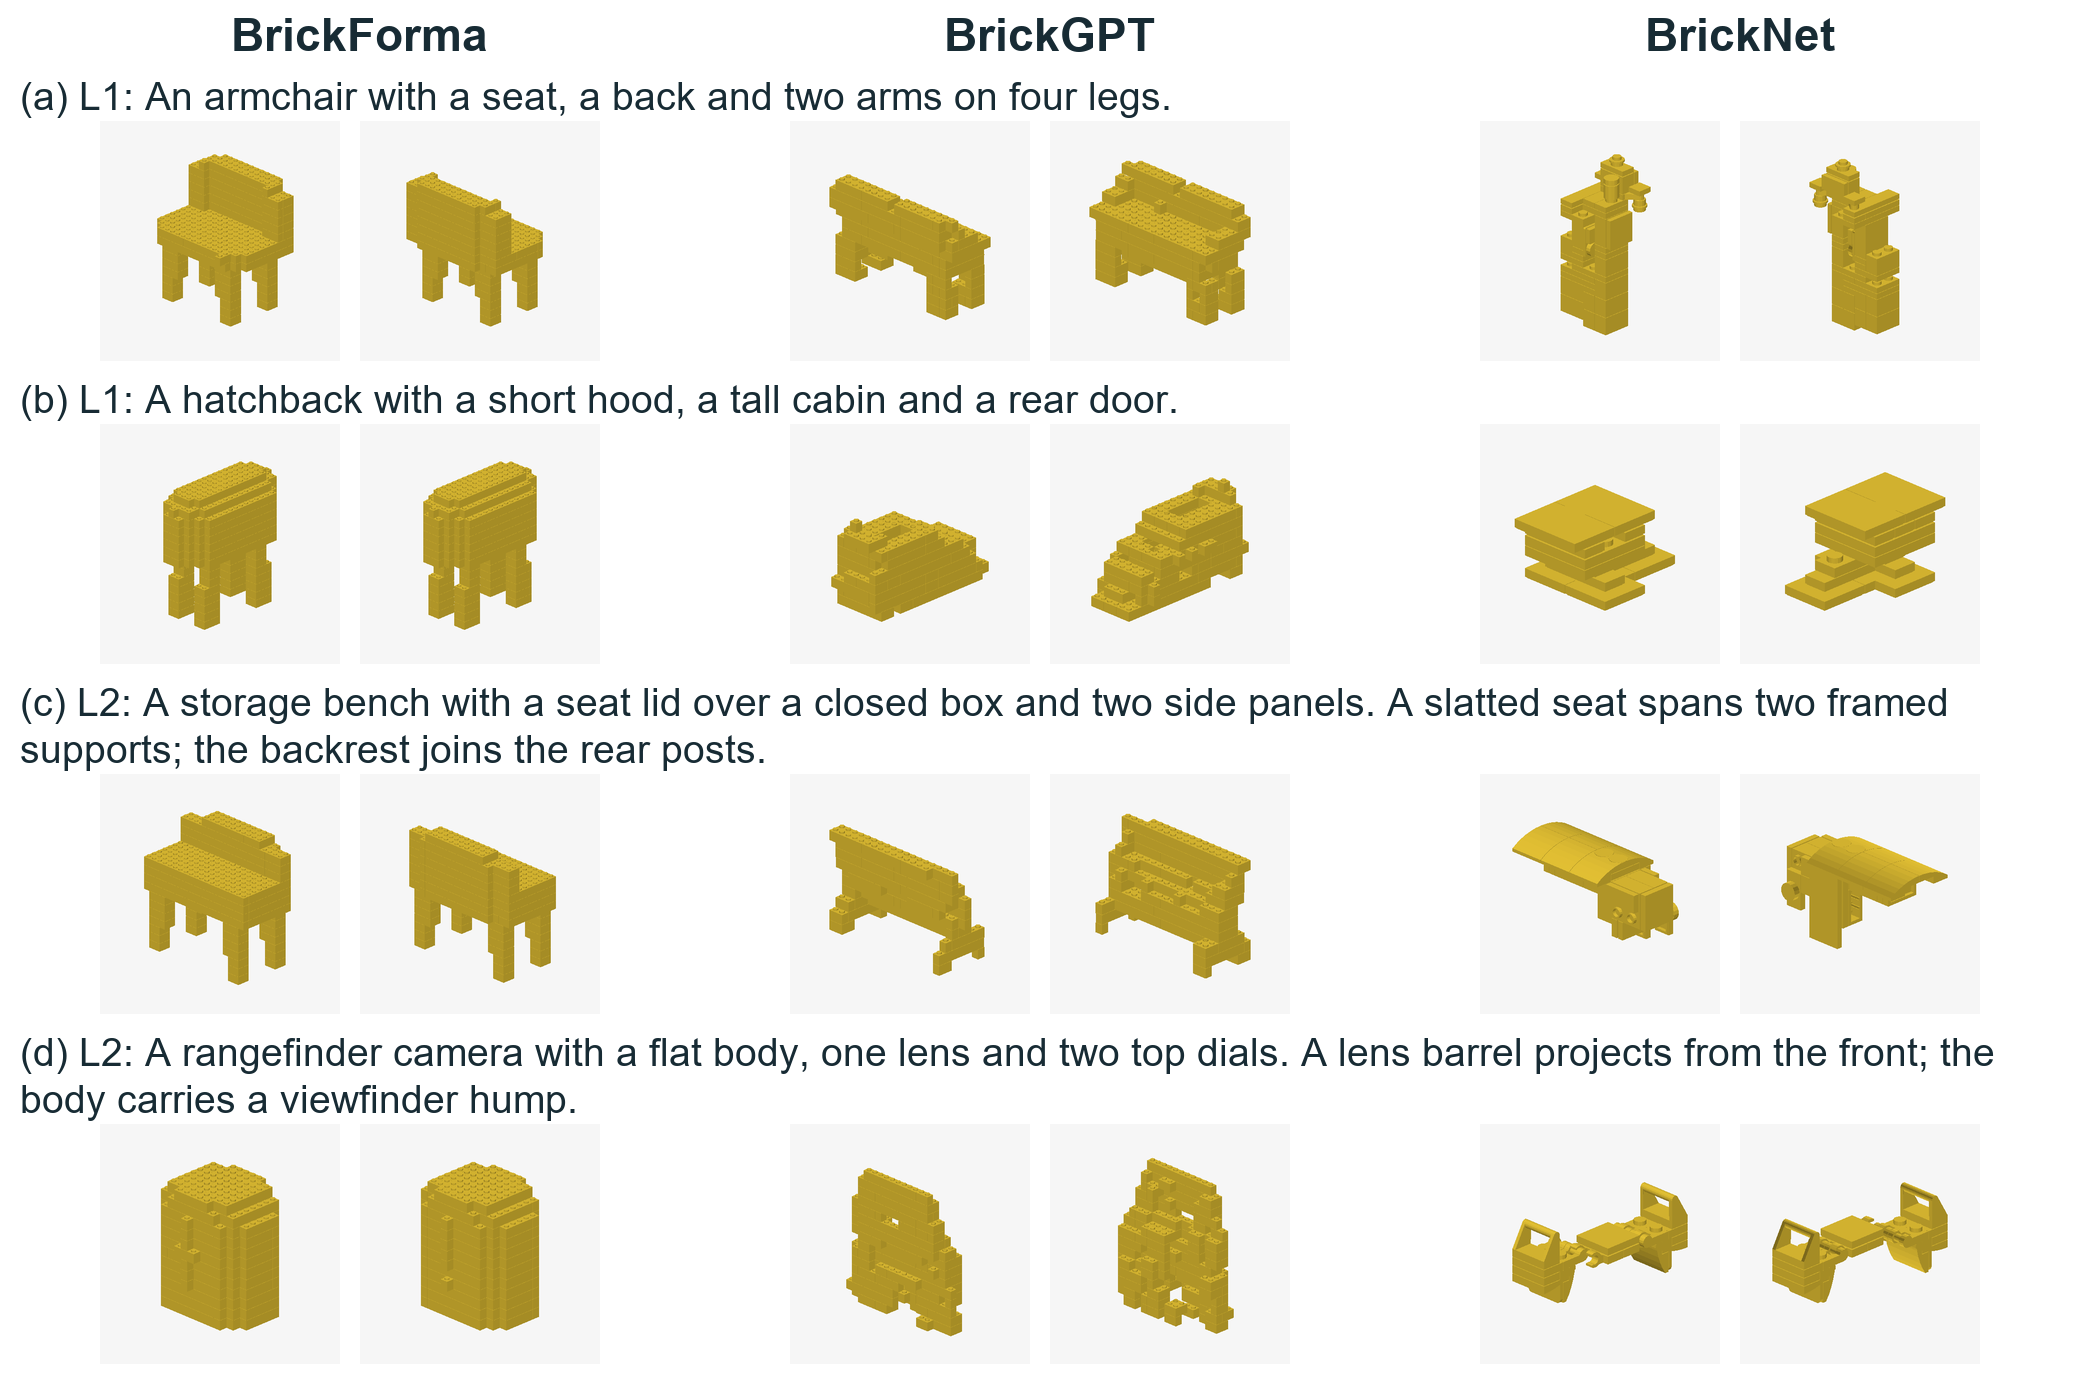
\includegraphics[width=\textwidth]{figures/matched_short_prompts_20261116.png}
\caption{Four matched Group B examples with the same prompts, render settings, and azimuths ($45^\circ$ and $225^\circ$) across systems. The highest VQAScore belongs to BrickForma for the chair and bench, BrickGPT for the hatchback, and BrickNet for the camera.}
\label{fig:gallery}
\end{figure*}


\subsection{Raw versus Retiled Outputs}
\begin{table}[t]
\centering
\small
\begin{tabular}{lrr}
\toprule
Metric & Raw & Retiled \\
\midrule
$P_{\mathrm{inv}}$ $\downarrow$ & 0.1897\% & 0.0000\% \\
VQAScore $\uparrow$ & 0.2065 & 0.2071 \\
PE $\uparrow$ & 0.1858 & 0.1859 \\
SigLIP2 $\uparrow$ & 0.1379 & 0.1261 \\
Mean parts & 178.7 & 421.2 \\
\bottomrule
\end{tabular}
\caption{Earlier repair comparison on 110 pairs sharing the same prompt, model identifier, and caption.}
\label{tab:raw-retiled}
\end{table}

We examine reconstruction on 110 raw/retiled pairs from an earlier 114-prompt comparison (Table~\ref{tab:raw-retiled}). Retiling reduces mean $P_{\mathrm{inv}}$ from 0.1897\% to 0.0000\% and increases mean part count from 178.7 to 421.2. VQAScore and PE change little, while SigLIP2 falls from 0.1379 to 0.1261. Each pair shares a prompt and model identifier.

\subsection{Geometric Reconstruction Audit}
\label{sec:diagnostics}
We define stud contacts by footprint overlap across adjacent layers. We map the same 110 pairs to a grid with 20 LDU horizontal pitch and 24 LDU layer height and translate each export to a common occupied-cell origin. All 110 pairs have equal occupied voxel unions after translation. Single-component layouts rise from 18 to 110, and overlap-free layouts rise from 100 to 110 (Table~\ref{tab:export-audit}).
\begin{table}[t]
\centering\small
\begin{tabular}{@{}lrr@{}}
\toprule
Export measure & Raw & Retiled \\
\midrule
Single stud component & 18/110 & 110/110 \\
Mean stud components & 4.29 & 1.00 \\
No body-cell overlap & 100/110 & 110/110 \\
\midrule
\multicolumn{3}{@{}l@{}}{Equal voxel unions after translation: 110/110} \\
\bottomrule
\end{tabular}
\caption{Earlier export audit of 110 matched raw/retiled pairs. Union equality uses translation normalization.}
\label{tab:export-audit}
\end{table}

In the separate 525-prompt diagnostic run, 46 raw layouts have a single stud component. All 525 final layouts form one component and preserve their corresponding target unions after the reported recovery procedure (Appendix~\ref{app:eval}).

\subsection{Evaluation Boundaries}
The comparison uses delivered exports from systems with different inference settings and part libraries. The description levels vary in both content and length. PE truncates 59 Group B prompts and SigLIP2 truncates 106 (Appendix~\ref{app:eval}). Uniform yellow rendering evaluates shape and layout without assessing color fidelity. The paired reconstruction audit describes the delivered selected pairs. Its denominator excludes unsuccessful solver attempts.

\section{Limitations and Discussion}
The program-based transfer combines generator design, geometric validation, and supervised fine-tuning. Isolating the contribution of large-model authoring would require an alternative generator evaluated under a matched training budget.

The dataset release checks grounding and coverage, and reconstruction enforces a single stud-connected component. Mechanical stability and a feasible assembly order require separate measurements. The integrated release and the training run record their counts separately (Table~\ref{tab:training-data}).

\section{Conclusion}
BrickForma converts program-generated voxels into checked brick layouts and uses them to fine-tune Qwen3-1.7B. Its raw outputs lead the three alignment metrics in aggregate on 265 matched prompts, with a mean invalid-placement ratio of 0.81\%. In the earlier paired audit, exact-cover reconstruction restores stud connectivity while preserving the occupied voxel union.
